\chapter{Kieker Analysis Component}\label{chap:componentsAnalysis}
	
	% Notify-tag; this is more or less a reminding.
	\class{\KiekerAnalysisPart} is the part of \Kieker\  which is responsible for the analysis, consisting of the reader, the consumer and the analysis instance itself. To read the stored records again is task of the readers. Whatever is done with these informations is task of the consumers. They can evaluate, process or visualize the data for example. The analysis instance concerns about the lifetime and registration of the other parts. As explained in the example chapter, the analysis consists\notify  of the following steps:
	\begin{enumerate}
		\item Create a new instance (or more) of the class \class{AnalysisInstance}.
		\item Register the plugins which should evaluate the records.
		\item Register exactly one reader to read the stored informations.
		\item Start the analysis instance.
	\end{enumerate}

	\section{Monitoring Log Readers}

		% Warning-tag for the reader-writer-thing
		The monitoring log readers are the direct counterpart to the monitoring log writers. While a writer gets a record and writes it into files or somewhere else, the reader takes the written data and converts it into a suitable instance of \class{AbstractKiekerMonitoringRecord}. \warning This means that whenever a new writer is implemented, a corresponding reader has to be implemented as well. If one want for example to store the recorded informations in a database, one should be capable of reading these saved informations from the database again.\\
		There are already some readers implemented in \Kieker\  as can be seen in the hierarchy diagram in Figure \ref{Figure:ReaderHierarchy}.

		% This image shows the reader hierarchy.
		\begin{figure}[H]
			\begin{centering}
				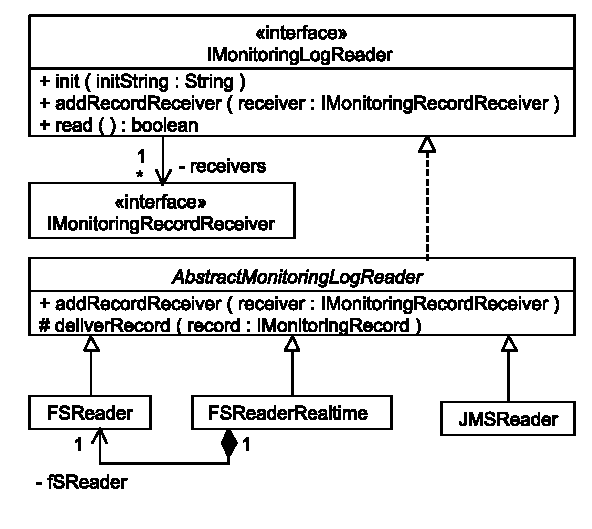
\includegraphics[width=0.5\textwidth]{images/kieker_readerimpls}
				\caption{The simple inheritance hierarchy of some currently implemented monitoring log readers}
				\label{Figure:ReaderHierarchy}
			\end{centering}
		\end{figure}

		The implementing of an own reader is nearly the same as the implementing of the writer, but to keep things simple, it is recommended to extend the already implemented AbstractKiekerMonitoringLogReader, because otherwise it would be necessary to implement the used observer pattern of the reader. By using the methods of the abstract class \class{kieker.analysis.reader.AbstractMonitoringLogReader}, the task of delivering a new record to the consumers can be delegated to the super class.\\
		The Listing \ref{listing:MyReader} shows a simple reader which reads a stored record from the pipe. If there is nothing on the pipe to be read, the reader waits 4 seconds at maximum before it terminates.

		\setJavaCodeListing
		\lstinputlisting[caption=MyReader.java, label=listing:MyReader]{\customComponentsBookstoreApplicationDir/src/bookstoreTracing/MyReader.java}

	\section{Record Consumer Plugins}

		The consumers are the parts of Kieker which work with the records that have been loaded by the reader. There can be (theoretically) an infinite number of consumers which produce any kind of output. A consumer can be programmed by implementing the interface \class{kieker.analysis.plugin.IMonitoringRecordConsumerPlugin} and writing the necessary methods. Following example consumer takes the given record and writes the content to the default output stream.

		\setJavaCodeListing
		\lstinputlisting[caption=MyConsumer.java]{\customComponentsBookstoreApplicationDir/src/bookstoreTracing/MyConsumer.java}

	\section{Analysis Instance}

		To put everything together, Listing \ref{listing:AnalysisInstance} shows how to use the above-mentioned components.

		\setJavaCodeListing
		\begin{lstlisting}[label=listing:AnalysisController]
AnalysisController ai = new AnalysisController();
MyReader reader = new MyReader(); 
reader.init("somePipe"); 
ai.setLogReader(reader); 	  ai.registerPlugin(new MyConsumer());
ai.run();
\end{lstlisting}
